%% $RCSfile: proj_report_outline.tex,v $
%% $Revision: 1.2 $
%% $Date: 2010/04/23 02:40:16 $
%% $Author: kevin $

\documentclass[11pt
              , a4paper
              , twoside
              , openright
              ]{report}


\usepackage{float} % lets you have non-floating floats
\usepackage{graphicx}
\usepackage{url} % for typesetting urls

%
%  We don't want figures to float so we define
%
\newfloat{fig}{thp}{lof}[chapter]
\floatname{fig}{Figure}

%% These are standard LaTeX definitions for the document
%%                            
\title{An Investigation into Alternative Solutions to ESPAC for Assessing Earthquake Liquefaction Potential}
\author{George Charles Davie}

%% This file can be used for creating a wide range of reports
%%  across various Schools
%%
%% Set up some things, mostly for the front page, for your specific document
%
% Current options are:
% [ecs|msor]              Which school you are in.
%
% [bschonscomp|mcompsci]  Which degree you are doing
%                          You can also specify any other degree by name
%                          (see below)
% [font|image]            Use a font or an image for the VUW logo
%                          The font option will only work on ECS systems
%
\usepackage[font,ecs,mcompsci]{vuwproject}
\supervisor{William Neil L Browne}

% You should specifiy your supervisor here with
%     \supervisor{Firstname Lastname}
% use \supervisors if there is more than one supervisor

% Unless you've used the bschonscomp or mcompsci
%  options above use
\otherdegree{Bachelor of Engineering with Honors (Software)}
% here to specify degree

% Comment this out if you want the date printed.
\date{}

\begin{document}

% Make the page numbering roman, until after the contents, etc.
\frontmatter

%%%%%%%%%%%%%%%%%%%%%%%%%%%%%%%%%%%%%%%%%%%%%%%%%%%%%%%

%%%%%%%%%%%%%%%%%%%%%%%%%%%%%%%%%%%%%%%%%%%%%%%%%%%%%%%

\begin{abstract}

Standard regression techniques for soil analysis are time consuming and subject to human bias. The Institute of Geological and Nuclear Sciences (GNS) and Victoria University have developed a proof of concept prototype as a solution to this problem, Evolutionary Spatial Auto-Correlation (ESPAC). ESPAC is an implementation of the parallel linear genetic programming (PLGP) algorithm. Due to the nature of this project no alternative solutions were investigated. This project aims to address this issue by investigating the properties of other Evolutionary Computation based artificial intelligence techniques. The aim to lend strength to the argument that PLGP is the correct solution to the problem, or find that an alternative method would be more viable.


\end{abstract}

%%%%%%%%%%%%%%%%%%%%%%%%%%%%%%%%%%%%%%%%%%%%%%%%%%%%%%%

\maketitle


\tableofcontents

% we want a list of the figures we defined
%\listof{fig}{Figures}

%%%%%%%%%%%%%%%%%%%%%%%%%%%%%%%%%%%%%%%%%%%%%%%%%%%%%%%

\mainmatter

%%%%%%%%%%%%%%%%%%%%%%%%%%%%%%%%%%%%%%%%%%%%%%%%%%%%%%%

% individual chapters included here
\chapter{Introduction}\label{C:intro}

Earthquakes are known to cause severe damage to human life and infrastructure. A significant portion of the problems associated with an earthquake event are due to ground instability. A developed site can have poor ground stability for a number of reasons. The one this body of work is addressing is liquefaction. Liquefaction occurs when sediments, silts and sands below the water table lose their structural strength during an earthquake. The sediments float within the compressed water causing the strength of the stratigraphic layer to fail. At which point it can no longer support the layers above it causing them to sink \cite{1}, \cite{2}.
\\\\
Techniques to determine the probability that a site will liquefy during an earthquake event have been around for a while. Most of these involve the study of core samples. These are destructive to the site, expensive and time consuming to obtain. However a technique called SPAC was developed to measure surface micro-tremors which significantly reduces the problems associated with the recovery of core samples \cite{2}, \cite{3}, \cite{5}, \cite{6}, \cite{7}. This process is still fairly labor intensive, though it can be done off-site, as it currently uses the simplex algorithm which requires a lot of human operator intervention. The simplex algorithm is used during the modeling of the data as part of an iterative process with the goal of finding the best fitness \cite{2}, \cite{7}. 
\\ \\
This project is building upon Aaron Scoble's work he submitted last year in completion of his summer project and honors research. His work examines the use of AI, specifically Parallel Linear Genetic Programming (PLGP) to solve the current human problems associated with the simplex algorithm \cite{scoble1}. Essentially the current simplex algorithm is very labor intensive and prone to human bias and assumption. Developing a processes that would provide accurate reliable results with a reduction in human processing time would be a beneficial tool to the geotechnic industry. The benefits an AI system could achieve include:
 
 \begin{itemize}
 \item • A reduction in the cost of site evaluations by lessening a geotechnic engineer’s (geotech’s) billable hours.
 \item • A reduction in the time to analyse the data, resulting in faster evaluations.
 \item • A more transparent result that is devoid of human bias, allowing greater client confidence.
 \end{itemize}

There are also several academic contributions that an AI solution could achieve, these include:

 \begin{itemize}
 \item • Improved regression analysis within hard and soft constraints.
 \item • An AI solution to an industry problem reinforcing the benefit of further AI research.
 \end{itemize}

Aaron's work investigates the use of parallel linear genetic programing (PLGP) to achieve these goals. This project uses his algorithm as a benchmark with which to test several other AI techniques in an effort to determine which are better suited to this particular regression problem. PLGP is a complex algorithm that does not lend itself to transparency nor has it seen much use in commercial projects. Using a more widely known and understood technique has the potential to be quicker to implement and maintain while providing a higher degree of client confidence. The outcome of this paper is not to have a polished industry ready solution but rather to have determined which direction would be most profitable for further research. 
\\\\
The success of each implementation will be measured as follows:


 \begin{itemize}
 \item Run speed of the implementations.
 \item Performance in the detection of potential liquefaction risks.
 \end{itemize}
 
 
 
%% $RCSfile: using.tex,v $
%% $Revision: 1.1 $
%% $Date: 2010/04/23 01:57:05 $
%% $Author: kevin $
%%
\chapter{Previous and Related Work}\label{C:us}




\section{Related Work}

\subsection{Spatial Auto-Correlation (SPAC)}
Soil liquefaction refers to the process of the saturation of unconsolidated sediments usually by water to the point which the sediments take on liquid like properties. This phenomenon is usually induced during an earthquake event. Sediments, silts and sands below the water table lose their structural strength during an earthquake as they compress the water filled spaces building up pressure to the point that the sediments start to float. At which point the soil layer can no longer support the material above it causing the surface layers to sink \cite{3} \cite{5} \cite{6}.
Spatial Auto-Correlation (SPAC) is a geophysical method that records micro tremors caused by Rayleigh waves to calculate the shear-wave velocity of a stratigraphic column. A low shear wave velocity through a soil layer indicates a very porous material that when submerged below the water table has a high potential to liquefy \cite{2} \cite{7} \cite{10}.

\begin{figure}[h]
\centering
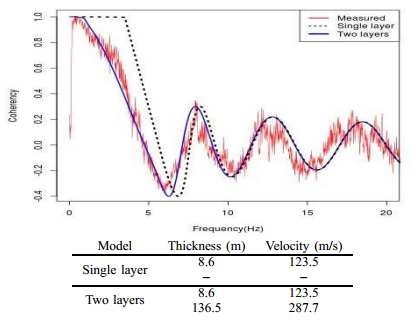
\includegraphics[width=100mm]{simplex.png}
\caption{GP program tree}
\centering
\end{figure}

\subsection{The Computer Programs in Seismology (CPS)}
The Computer Programs in Seismology (CPS) is a software suite containing a number of modules that are able to analyse seismic data like the measured Rayleigh wave data collected using the SPAC method \cite{11}. The suit contains a model of the earths stratigraphic data, specifically, approximate thickness and shear wave velocity data. The modal summation software module calculates a dispersion curve which is then passed to an inversion process, resulting in a theoretical coherency curve which is matched for errors against the data obtained in the field.



\subsection{Simplex Algorithm}
For any linear programming problems the Simplex algorithm is able to deliver a solution. This is the method that is currently used by Geo-technical Engineers in determining the best fit with the theoretical coherency function \cite{2}. The Simplex algorithm with the aid of an operator continuously calls the CPS suit refining the model until no further improvements can be made. It is this process that is slow, time consuming and currently requires heavy human involvement. Figure 2.1 shows a curve being refined with the addition of a second layer.



\subsection{Genetic Programming for Symbolic Regression}
When a model of the curve of best fit is the required objective of a problem you have a regression problem. Therefore as we are using a measured coherency as our target and are creating theoretical coherency curves using the CPS suite we have a regression problem \cite{13} \cite{scoble1}. The accuracy of this theoretical curve against the measured coherency of specific sites is the fitness function for our evolutionary processes.


\subsection{Genetic Programming (GP)}
Genetic programming (GP) is an evolutionary algorithm that given data and a fitness function mutates a function to produce a fitness result. This nature makes it an ideal candidate for regression problems \cite{poli1} \cite{scoble1}. Each evolution of the program is matched against the fitness function and using an elitism technique a subset of the total population is mutated into a new population. Typically a GP programs runs with a tree like structure as can be seen in figure 2.2 \cite{13}. This continues for a predetermined number of cycles and the results of the final elitism selection are returned.

\begin{figure}[h]
\centering
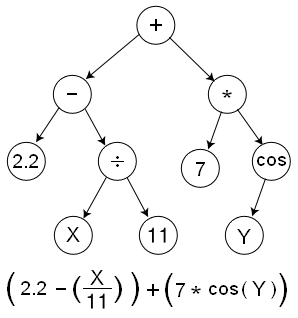
\includegraphics[width=40mm]{Genetic_Program_Tree.png}
\caption{GP program tree}
\centering
\end{figure}



\subsection{Linear Genetic Programming (LGP)}
Linear genetic programming (LGP) is similar in its operation to GP however rather than the tree structures that the GP produces, LGP has a graph based functional structure. This means that previously executed populations are able to be recycled into generations other than their direct children. While this is powerful it does mean minor changes to previous populations can cascade down to younger generations, which can cause large disruptions in the data \cite{poli1} \cite{16} \cite{17}. 


\subsection{Parallel Linear Genetic Programming (PLGP)}
Parallel linear genetic programming (PLGP) limits the dependencies the instructions have between one another. PLGP essentially has a number of LGPs that run separately to one another. Crossovers and mutations are made across the LGPs rather than vertically over themselves. This limits the mutations to equivalent generations. The results is subpopulations that may mutate within themselves but not between populations. Upon completion the final results are added together across the LGPs \cite{15} \cite{22} \cite{23} \cite{24}.


\section{Previous Work}
\subsection{Aaron Scoble's Contribution}

Aaron Scoble successfully implemented the ESPAC system to solve a real world regression task. This achievement was a first and major contribution for PLGP \cite{scoble1}. The problem itself was to create a model that could reliably estimate the liquefaction potential of a specific site during an earthquake event using an autonomous process. The benefits and reasons for this work have previously been outline within Chapter \ref{C:intro}.

Aaron's work used a number of assumptions and simplifications that will be carried over to this project due to the scope. However it needs to be noted that these need to be addressed before any of the techniques can be commercially deployed. The main three are:


 \begin{itemize}
 \item A fixed value of 2 for the number of layers present within each experiment. Aaron suggests a possible solution to this within his work.
 \item The assumption that each of these layers are perfectly horizontal and that no folding or other type of geological deformation has occurred.
 \item The assumption that libCPS and CPS are functioning correctly and are current.
 \end{itemize}
 
 Another major contribution of Aaron's work is the libCPS library that successfully wraps the existing CPS modal summation module into a Java Native Interface (JNI) library \cite{scoble1}. This will be used through each of the Java AI implementations within the project.


\chapter{Progress}\label{C:ex}


\section{Geological Background}
During the mid-semester break there was a trip to Nelson as part of an introductory field geology paper, ESCI-241. The relevancy of this exercise was to conceptualize the gathered data the various AI techniques would be working upon. This trip gave a lot of insight into understanding the scale of various stratigraphic layers and their composition. It also brought up a number of points that are out of scope for this project but will need addressing before any of the proposed solutions are industry ready.


The main point being that the contact between layers is rarely horizontal. Over an aperture distance of 20-30 meters the reading of these contacts would become distorted, producing data that is hard to accurately model using the proposed AI solutions. This problem exists within the current human operated simplex method but an experienced technician will have relevant structural background to understand these features that the AI solutions would find hard to model.  This leads further credence to the need to fix a number of simplifications used within previous work.


Another generalization that this work and previous work uses is that there are only ever two layers. This excursion demonstrated that while there are often only one or two layers that would have an effect on the surface layer, the current work still does not support this variance. Examples of a number of sites that had more than 2 layers were also witnessed. This is the easier of the two generalization to amend. 
\section{Implementation of Existing Work}
A major achieved milestone was the handover of the existing work and the familiarization with the system to the point where the past experiments can be repeated. This has involved updating the existing implementation to work on the updated ECS system that is now running Java 7 rather than 6. A refactoring of several duplicated classes has occurred to make the system more readable and allow the extraction of the libCPS library. Scripts have been successfully written to allow batch testing and experiment duplication over the grid.

\section{Benchmark Data Acquisition}

In order to successfully compare the different AI methods a substantial amount of data needs to be collected. The data that Aaron collected from the PLGP is not sufficient to fairly contrast the other techniques against. Due to time constraints and the slow nature of libCPS, generations were limited to 50. The oscillation phenomena Aaron experienced may be reducible using a larger number of generations \cite{scoble1}.


Aaron acknowledges his work as a proof of concept and does not provide rigorous testing of the ESPAC technique. So a new step within the project has to be to gather a set of statistically strong data. There were a number of decisions related to the configuration of these experiments that needed to be made. As the best operational conditions have yet to be determined for the PLGP implementation additional experiments to contrast a number of different run configurations need to occur. The next section details the following experiments that have been run or are in the process of running to fulfill this.

\section{PLGP Results}

Still waiting on more grid results before the data can be empirically evaluated. Once these results are in a study of the data using both Student's paired sample t-tests and Wilcoxon rank-sum test will be conducted.



\subsection{Population 100 with 80 Generations}
This was the first experiment to have a significant number of runs, 30, on the grid. The numbers were chosen with a focus on determining the speed at which the program executed. These runs took on average 22 hours to complete.
\\\\
The graphs in Figure 3.1 show a cross section of the data collected for the PLGP running with a population of 100 with 80 generations. It is expected that the variance is due to the small population size and that decreasing the number of generations by half will have little effect on the fitness.


\begin{figure}[h]
{\begin{center}
\begin{tabular}{ll}
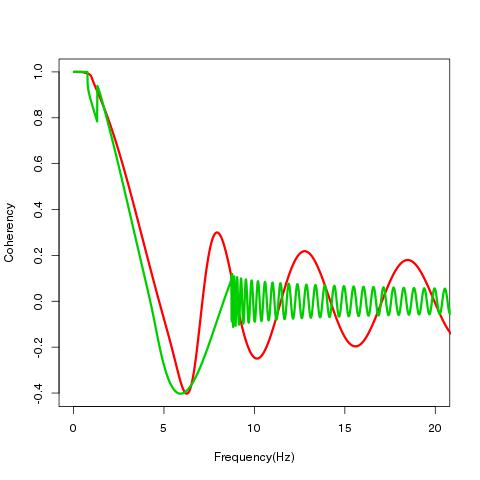
\includegraphics[width=80mm]{pop1003.jpg} & 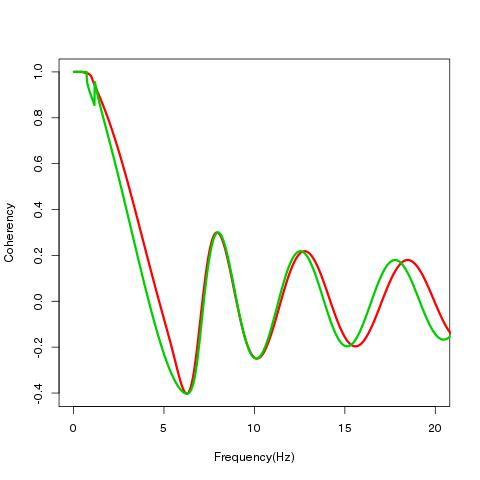
\includegraphics[width=80mm]{pop1002.jpg}
\end{tabular}
\caption{Two graphs highlighting the variance found within 30 runs of the PLGP with a population of 100 and 80 generations}
\end{center}}
\end{figure}
\clearpage

\subsection{Population 100 with 40 Generations}

The purpose of this experiment is to determine the difference found between changing the number of generations over a small population.
\\\\
Results Pending

\subsection{Population 1000 with 40 Generations}
The purpose of this experiment is to determine the difference found between changing the population and to determine the speed of the application. The average run time for these was 4.8 days.
\\\\
The graphs in Figure 3.2 show a cross section of the data collected for the PLGP running with a population of 1000 with 40 generations. The variance seen here is very similar to that seen with a population of 100 and 80 generations. As we proposed that 100 populations with 40 generations would be similar this indicates our smallest set of runs is providing an optimal solution given the current fitness function.



\begin{figure}[h]
{\begin{center}
\begin{tabular}{ll}
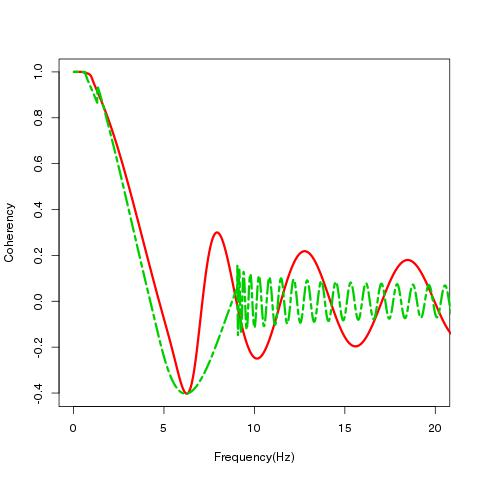
\includegraphics[width=80mm]{pop10001.jpg} & 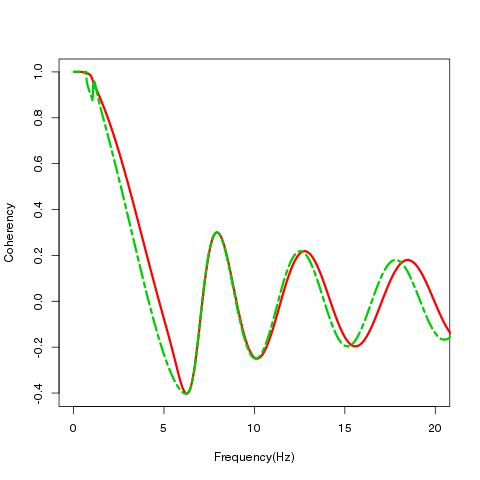
\includegraphics[width=80mm]{pop10003.jpg}
\end{tabular}
\caption{Two graphs highlighting the variance found within 30 runs of the PLGP with a population of 1000 and 40 generations}
\end{center}}
\end{figure}
\subsection{Population 1000 with 80 Generations}
The purpose of this experiment is to satisfy our hypothesis that a population of 1000 with 80 generations will have the same variance and local optimization as a run with a population of 100 with 40 generations.
\\\\
Still waiting on grid results before this hypothesis can be evaluated.



\section{GA Implementation}

A basic GA has been implemented following a number of ECJ tutorials. The purpose of this was to gain an understanding of the library before attempting the full GP. The GA is fairly basic and not suited to the regression problem so out side of this exercise it will not be used or test.

\section{GP Implementation}

Currently just the ECJ tutorial has been implemented. A full implementation of the GP is the next major hurdle that will be accomplished.

\chapter{Plans}\label{C:con}

\section{Proposal Review}

\subsection{Stage 1} 
This will primarily be research into the problem itself.This includes the physical
science behind it and the algorithms mentioned above. While a portion of this will be
continuous throughout the project the bulk should be completed by 22 April with a
presentation given to GNS around this time.
\\\\
Completed but presentation has yet to be given but will be arranged at a time convenient to GNS.

\subsection{Stage 2} 
Each of the above techniques will then be further investigated to determine their fit for the proposed problem. This is to remove any redundancy and avoid complication during stage 3. This should be completed by 10 May with the completion of a one page report.
\\\\
Completed - work can be found within background section.

\subsection{Stage 3} 
The third task will be determining the evaluation methods used to benchmark the
success of each technique. A fitness function for the given problem will be determined
using the pre-existing work and communication with a geotech at GNS. This should
be completed by 19 July by GNS acceptance of the documented methods.
\\\\
This has changed as the fitness function will be the same as that found within Aaron's work. However the collection of benchmark data from Aaron's work has commenced. This will be completed by the 21st of June.

\subsection{Stage 4} 
The techniques that meet the problems criteria will then be developed in Java and
tested against existing benchmarks/standards a number of times to ensure statistical
confidence. These results will be collated into an appendix by 8 September, this will
be attached to the final report.
\\\\
The implementation of these techniques will be completed by 15 July.

\subsection{Stage 5} 
The evaluation techniques that were developed during stage 3 will then be tested
against the remaining algorithms and the existing parallel linear genetic programming
solution. Again these tests will be run multiple times to ensure statistical confidence
and be written into an appendix by 27 September.



\subsection{Stage 6} 
The final stage will be to ensure all the resources used and developed during the
project are in a presentable format. This includes a written report, oral presentation
and a tidy code repository for any future work.
\\\\
Written Report - 18 October
\\
Oral Presentation - 16 November
\\
Tidy Code Repository - 16 November

\section{Gantt Chart}

\begin{figure}[h]
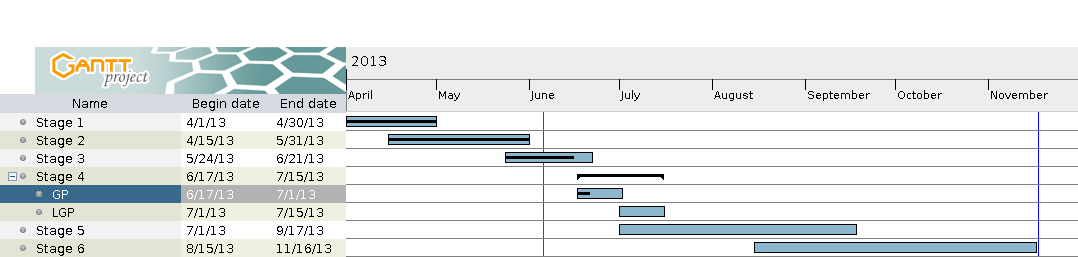
\includegraphics[width=170mm]{ganttV1.png}
\caption{Gantt Chart Created 3 June 2013}
\end{figure}

\section{AI Libraries}
Rather than reinventing the wheel there already exist a number of Java libraries built specifically for the implementation of genetic programming programs. Within Victoria University there has been a substantial amount of work done using the ECJ library. Due to this background and the amount of documentation available this will be used in the creation of the GP. There are currently no open source Java LGP libraries. Slash-A is the only out of the box LGP supporting library that has been developed and released but this is written in C++ and creating a new libCPS wrapper would be redundant. Carlton Downey has produced a Java LGP but it is currently not in the public domain. If this software cannot be obtained a LGP library will be built specifically for this research.
 
\chapter{Summary}\label{C:sum}

\section{Achievements to Date}

There have been a number of achievements to date. All of the background material has been covered and researched. This included research on existing software libraries and evaluating which ones are most likely to fit the problem. The best solutions that are currently available are the George Mason University's GP package named, ECJ and Carlton Downey's LGP library if this can be obtained. 


Aaron Scoble's existing work has been handed over and modified to work on a slightly different architecture. Benchmark data from this is being gathered and is near completion with a wait on a number of grid jobs awaiting that are still executing. 


\section{Major Hurdles Remaining}
There is a significant amount of work left within the project with the next major hurdle being the implementation of the GP. This will be closely followed by the implementation of the LGP. Once these are complete experiments will be run to determine each of the algorithms most efficient operating parameters. Data will then be collected with a heavy reliance on the ECS grid system. Once all this data is collected a statistical evaluation of the results will be written into a report. This report will become the results and discussion sections of the final write up which will be completed by the end of the year. 


\section{Contribution Goals}
The contributions of the project will be an implementation of both a GP and LGP used to determine the liquefaction potential of horizontal 2 layered stratigraphic records obtained during a site investigation using the SPAC system. These two systems will also be used in a study also featuring the PLGP to determine which of the three techniques is the most successful at solving the problem of liquefaction potential detection.



%%%%%%%%%%%%%%%%%%%%%%%%%%%%%%%%%%%%%%%%%%%%%%%%%%%%%%%

\backmatter

%%%%%%%%%%%%%%%%%%%%%%%%%%%%%%%%%%%%%%%%%%%%%%%%%%%%%%%


\bibliographystyle{ieeetr}
\nocite{*}
%\bibliographystyle{acm}
\bibliography{sample}


\end{document}